
%%----------------------------------------%%
\begin{frame}
  \frametitle{Heat Contributors In PWR SNF}
\footnotesize{
  \begin{figure}[htbp!]
  \begin{center}
    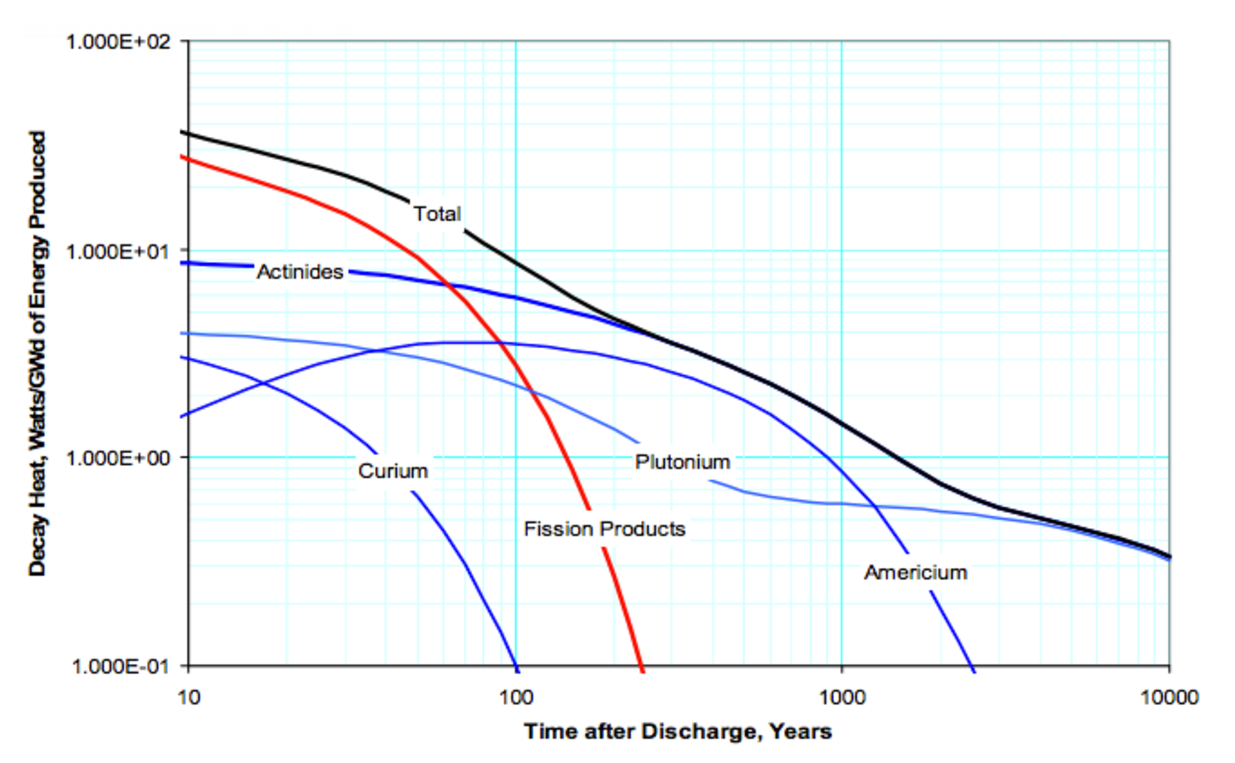
\includegraphics[width=0.7\textwidth]{./images/wigeland_heat.eps}
  \end{center}
  \caption{Heat contributors in a canonical PWR 
    fuel\cite{wigeland_relationship_2010}.}
  \label{fig:<++>}
\end{figure}

}
\end{frame}

%%----------------------------------------%%
\begin{frame}
  \frametitle{Heat Contributors in PWR SNF}
\footnotesize{
  \begin{figure}[htbp!]
  \begin{center}
    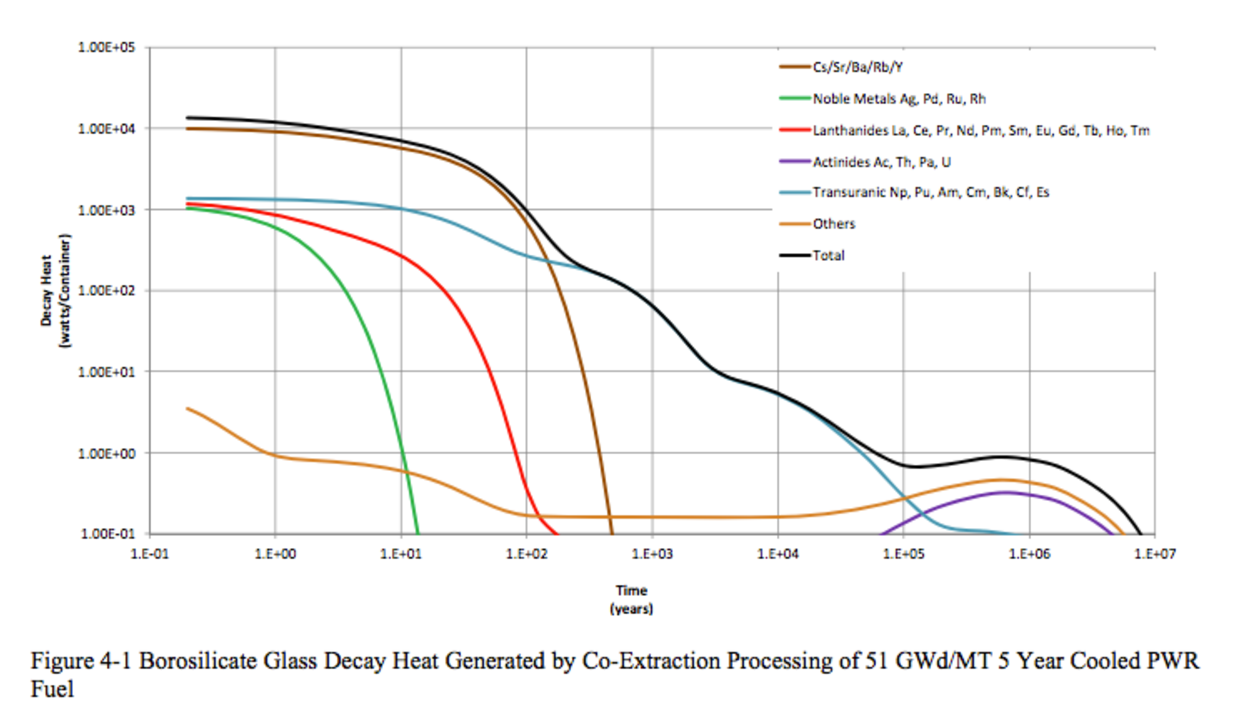
\includegraphics[width=0.7\textwidth]{./images/carter_coex_heat.eps}
  \end{center}
  \caption{Heat contributors in the primary result of a once through PWR fuel 
    cycle \cite{carter_us_2011}.}
  \label{fig:carter_coex_heat}
\end{figure}

}
\end{frame}
%%----------------------------------------%%
\begin{frame}
  \frametitle{Heat Contributors in LWR Recycled MOX}
\footnotesize{
  \begin{figure}[htbp!]
  \begin{center}
    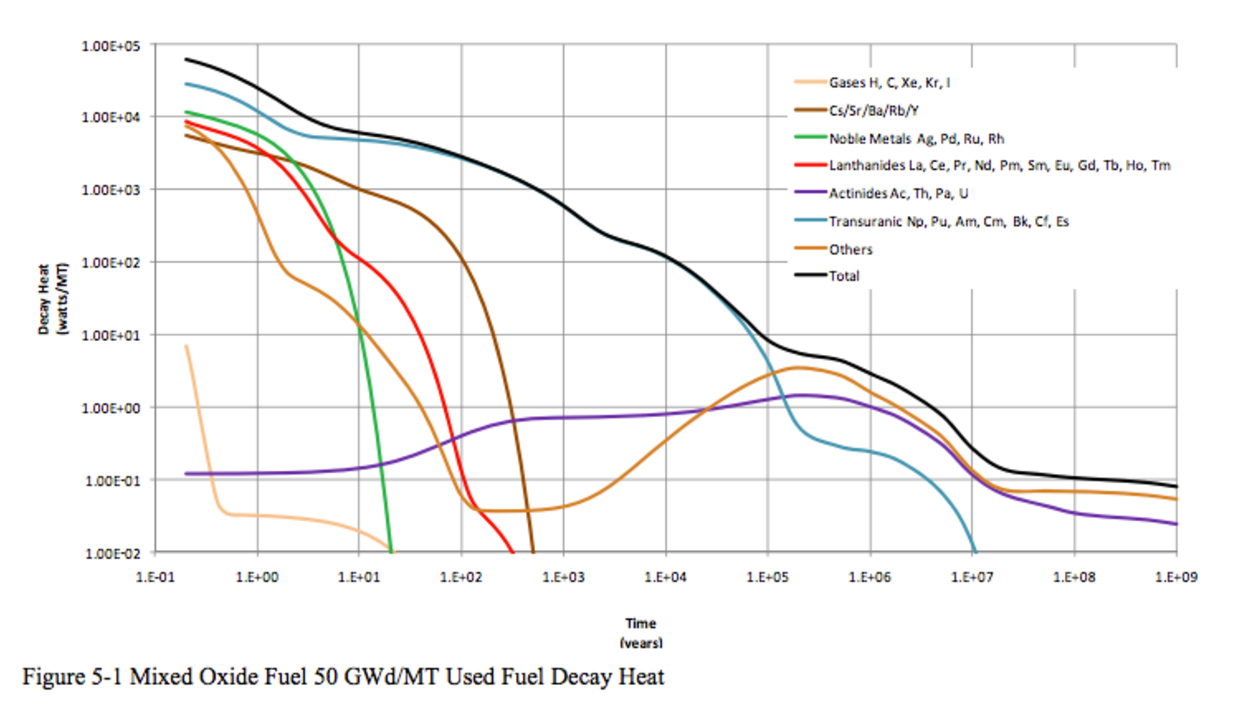
\includegraphics[width=0.7\textwidth]{./images/carter_lwr_mox_heat.eps}
  \end{center}
  \caption{Heat contributors in the primary result of MOX recycling in an LWR
    \cite{carter_us_2011}.}
  \label{fig:carter_lwr_mox_heat}
\end{figure}

}
\end{frame}
%%----------------------------------------%%
\begin{frame}
  \frametitle{Heat Contributors After NUEX Recycling}
\footnotesize{
  \begin{figure}[htbp!]
  \begin{center}
    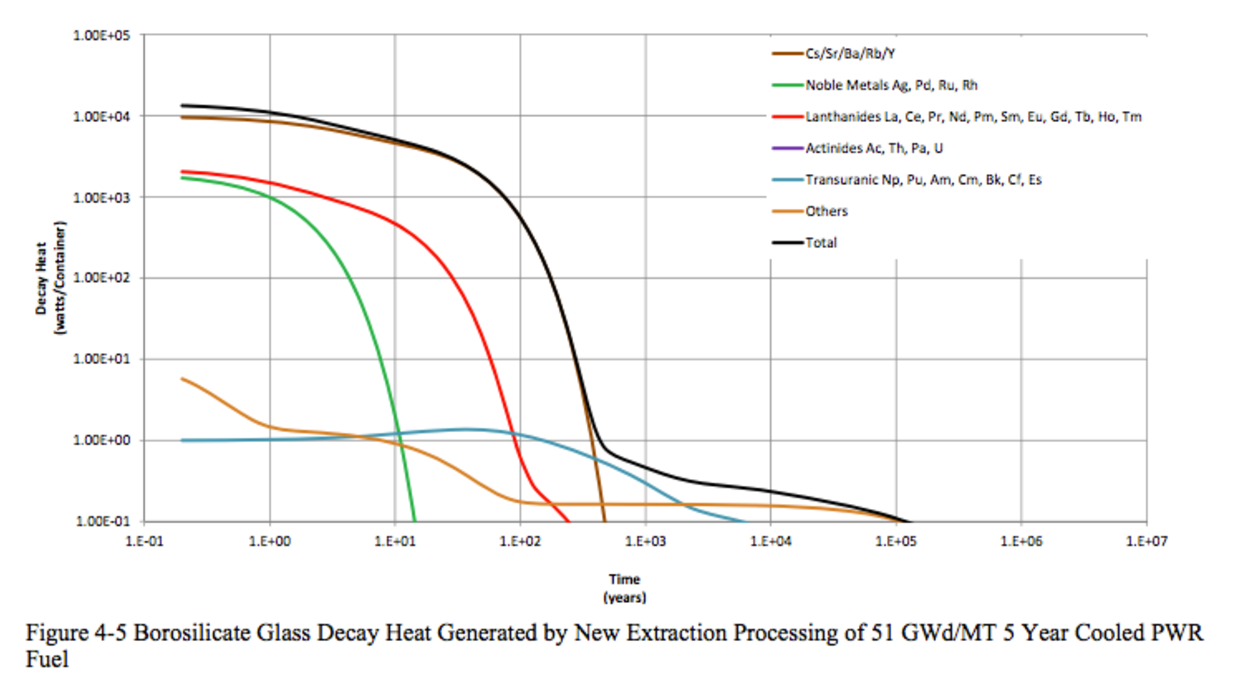
\includegraphics[width=0.7\textwidth]{./images/carter_nuex_heat.eps}
  \end{center}
  \caption{Heat contributors in the primary result of the NUEX extraction 
    process\cite{carter_us_2011}.}
  \label{fig:carter_nuex_heat}
\end{figure}

}
\end{frame}

%%----------------------------------------%%
\begin{frame}
  \frametitle{Heat Contributors After COEX Recycling}
\footnotesize{
  \begin{figure}[htbp!]
  \begin{center}
    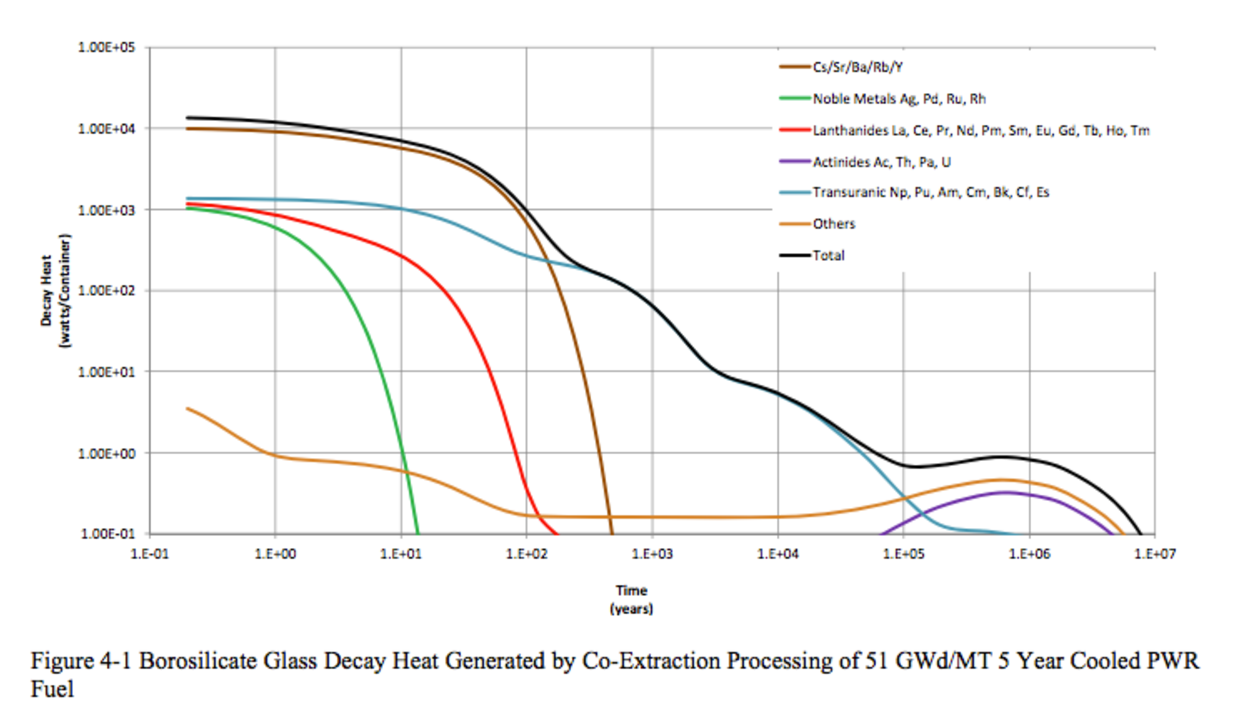
\includegraphics[width=0.7\textwidth]{./images/carter_coex_heat.eps}
  \end{center}
  \caption{Heat contributors in the primary result of the COEX extraction 
    process\cite{carter_us_2011}.}
  \label{fig:carter_coex_heat}
\end{figure}

}
\end{frame}
%%----------------------------------------%%
\begin{frame}
  \frametitle{Summary: Heat Contributing Isotopes in Various Fuel Cycles}
Dominant thermal contributors vary among fuel cycles. 
\begin{itemize}
   \item Recycling schemes are likely to reduce transuranics and actinides.
   \item Fission products such as Cs and Sr are powerful heat contributors in 
     the first 500 years, when capacity limiting peak heat is likely to occur in 
     many geologies.
   \item Transuranics, Pu, Np, Am, and Cm are dominant long term heat contributors. Some extraction processes are more successful at removing those from the waste stream. 
\end{itemize}
\end{frame}
